% Standalone didactic analysis of AES-128 and SM4.
% Build with:  python make_analysis.py   (from the repository root)
% The data file analysis/data.tex is generated from src/aes.py and src/sm4.py.
\documentclass[11pt,a4paper]{article}
\usepackage[T1]{fontenc}
\usepackage[utf8]{inputenc}
\usepackage[english]{babel}
\usepackage{lmodern}
\usepackage[margin=2.2cm]{geometry}
\usepackage{amsmath,amssymb,booktabs,xcolor,float,hyperref}
\usepackage{tikz}
\usepackage{pgfplots}
\pgfplotsset{compat=1.17}
\usetikzlibrary{arrows.meta,positioning,shapes.geometric,fit,backgrounds}

\hypersetup{colorlinks=true,linkcolor=blue!50!black,urlcolor=blue!50!black}

% Cell macro used by the generated S-box heatmaps: column, row, blue shade, hex.
\newcommand{\sbc}[4]{%
  \fill[blue!#3] (#1,-#2) rectangle +(1,-1);
  \node[font=\tiny\ttfamily,text=black] at (#1+0.5,-#2-0.5) {#4};}

% TikZ styles for the structure diagrams.
\tikzset{
  op/.style={draw,rounded corners,minimum width=3.4cm,minimum height=0.7cm,fill=blue!8,font=\small},
  io/.style={draw,rounded corners,minimum width=3.4cm,minimum height=0.7cm,fill=green!10,font=\small\bfseries},
  keyb/.style={draw,rounded corners,minimum width=1.9cm,minimum height=0.6cm,fill=orange!15,font=\footnotesize},
  flow/.style={-{Stealth[length=2mm]},thick},
}

% Auto-generated by make_analysis.py. Do not edit by hand.
\def\AEScipher{69C4E0D86A7B0430D8CDB78070B4C55A}
\def\SMfourcipher{536E424686B3E94FD206965E681EDF34}
\def\AESfixed{none}
\def\SMfourfixed{0xAB (171)}
\def\AESbitsreached{17}
\def\AESbitsfull{64}
\def\AESavalanche{(0,1)(1,17)(2,64)(3,65)(4,64)(5,70)(6,71)(7,58)(8,66)(9,71)(10,62)}
\def\AESbytes{(0,1)(1,4)(2,16)(3,16)(4,16)(5,16)(6,16)(7,16)(8,16)(9,16)(10,16)}
\def\SMfouravalanche{(1,1)(2,11)(3,31)(4,49)(5,63)(6,69)(7,67)(8,66)(9,67)(10,62)(11,64)(12,59)(13,56)(14,65)(15,57)(16,66)(17,66)(18,64)(19,73)(20,69)(21,77)(22,70)(23,61)(24,61)(25,52)(26,56)(27,58)(28,58)(29,61)(30,58)(31,61)(32,58)}
\def\AESsboxgrid{%
\sbc{0}{0}{42}{63}
\sbc{1}{0}{50}{7C}
\sbc{2}{0}{48}{77}
\sbc{3}{0}{50}{7B}
\sbc{4}{0}{86}{F2}
\sbc{5}{0}{45}{6B}
\sbc{6}{0}{46}{6F}
\sbc{7}{0}{72}{C5}
\sbc{8}{0}{27}{30}
\sbc{9}{0}{12}{01}
\sbc{10}{0}{44}{67}
\sbc{11}{0}{25}{2B}
\sbc{12}{0}{90}{FE}
\sbc{13}{0}{78}{D7}
\sbc{14}{0}{64}{AB}
\sbc{15}{0}{48}{76}
\sbc{0}{1}{74}{CA}
\sbc{1}{1}{52}{82}
\sbc{2}{1}{73}{C9}
\sbc{3}{1}{50}{7D}
\sbc{4}{1}{88}{FA}
\sbc{5}{1}{39}{59}
\sbc{6}{1}{34}{47}
\sbc{7}{1}{85}{F0}
\sbc{8}{1}{65}{AD}
\sbc{9}{1}{77}{D4}
\sbc{10}{1}{62}{A2}
\sbc{11}{1}{66}{AF}
\sbc{12}{1}{60}{9C}
\sbc{13}{1}{62}{A4}
\sbc{14}{1}{47}{72}
\sbc{15}{1}{71}{C0}
\sbc{0}{2}{68}{B7}
\sbc{1}{2}{89}{FD}
\sbc{2}{2}{57}{93}
\sbc{3}{2}{24}{26}
\sbc{4}{2}{29}{36}
\sbc{5}{2}{31}{3F}
\sbc{6}{2}{88}{F7}
\sbc{7}{2}{74}{CC}
\sbc{8}{2}{28}{34}
\sbc{9}{2}{62}{A5}
\sbc{10}{2}{82}{E5}
\sbc{11}{2}{86}{F1}
\sbc{12}{2}{47}{71}
\sbc{13}{2}{78}{D8}
\sbc{14}{2}{27}{31}
\sbc{15}{2}{18}{15}
\sbc{0}{3}{13}{04}
\sbc{1}{3}{73}{C7}
\sbc{2}{3}{23}{23}
\sbc{3}{3}{72}{C3}
\sbc{4}{3}{19}{18}
\sbc{5}{3}{58}{96}
\sbc{6}{3}{14}{05}
\sbc{7}{3}{59}{9A}
\sbc{8}{3}{14}{07}
\sbc{9}{3}{18}{12}
\sbc{10}{3}{51}{80}
\sbc{11}{3}{81}{E2}
\sbc{12}{3}{84}{EB}
\sbc{13}{3}{24}{27}
\sbc{14}{3}{66}{B2}
\sbc{15}{3}{48}{75}
\sbc{0}{4}{15}{09}
\sbc{1}{4}{52}{83}
\sbc{2}{4}{25}{2C}
\sbc{3}{4}{20}{1A}
\sbc{4}{4}{20}{1B}
\sbc{5}{4}{46}{6E}
\sbc{6}{4}{40}{5A}
\sbc{7}{4}{61}{A0}
\sbc{8}{4}{37}{52}
\sbc{9}{4}{30}{3B}
\sbc{10}{4}{77}{D6}
\sbc{11}{4}{67}{B3}
\sbc{12}{4}{25}{29}
\sbc{13}{4}{81}{E3}
\sbc{14}{4}{26}{2F}
\sbc{15}{4}{52}{84}
\sbc{0}{5}{37}{53}
\sbc{1}{5}{76}{D1}
\sbc{2}{5}{12}{00}
\sbc{3}{5}{84}{ED}
\sbc{4}{5}{22}{20}
\sbc{5}{5}{89}{FC}
\sbc{6}{5}{66}{B1}
\sbc{7}{5}{40}{5B}
\sbc{8}{5}{44}{6A}
\sbc{9}{5}{74}{CB}
\sbc{10}{5}{70}{BE}
\sbc{11}{5}{29}{39}
\sbc{12}{5}{35}{4A}
\sbc{13}{5}{35}{4C}
\sbc{14}{5}{39}{58}
\sbc{15}{5}{75}{CF}
\sbc{0}{6}{76}{D0}
\sbc{1}{6}{85}{EF}
\sbc{2}{6}{64}{AA}
\sbc{3}{6}{89}{FB}
\sbc{4}{6}{32}{43}
\sbc{5}{6}{36}{4D}
\sbc{6}{6}{28}{33}
\sbc{7}{6}{53}{85}
\sbc{8}{6}{33}{45}
\sbc{9}{6}{88}{F9}
\sbc{10}{6}{13}{02}
\sbc{11}{6}{51}{7F}
\sbc{12}{6}{36}{50}
\sbc{13}{6}{30}{3C}
\sbc{14}{6}{61}{9F}
\sbc{15}{6}{63}{A8}
\sbc{0}{7}{37}{51}
\sbc{1}{7}{62}{A3}
\sbc{2}{7}{32}{40}
\sbc{3}{7}{56}{8F}
\sbc{4}{7}{57}{92}
\sbc{5}{7}{60}{9D}
\sbc{6}{7}{29}{38}
\sbc{7}{7}{87}{F5}
\sbc{8}{7}{70}{BC}
\sbc{9}{7}{68}{B6}
\sbc{10}{7}{79}{DA}
\sbc{11}{7}{22}{21}
\sbc{12}{7}{17}{10}
\sbc{13}{7}{90}{FF}
\sbc{14}{7}{86}{F3}
\sbc{15}{7}{76}{D2}
\sbc{0}{8}{75}{CD}
\sbc{1}{8}{16}{0C}
\sbc{2}{8}{18}{13}
\sbc{3}{8}{84}{EC}
\sbc{4}{8}{41}{5F}
\sbc{5}{8}{58}{97}
\sbc{6}{8}{33}{44}
\sbc{7}{8}{19}{17}
\sbc{8}{8}{72}{C4}
\sbc{9}{8}{63}{A7}
\sbc{10}{8}{51}{7E}
\sbc{11}{8}{31}{3D}
\sbc{12}{8}{43}{64}
\sbc{13}{8}{40}{5D}
\sbc{14}{8}{20}{19}
\sbc{15}{8}{47}{73}
\sbc{0}{9}{41}{60}
\sbc{1}{9}{51}{81}
\sbc{2}{9}{36}{4F}
\sbc{3}{9}{79}{DC}
\sbc{4}{9}{22}{22}
\sbc{5}{9}{25}{2A}
\sbc{6}{9}{56}{90}
\sbc{7}{9}{54}{88}
\sbc{8}{9}{33}{46}
\sbc{9}{9}{85}{EE}
\sbc{10}{9}{68}{B8}
\sbc{11}{9}{18}{14}
\sbc{12}{9}{80}{DE}
\sbc{13}{9}{41}{5E}
\sbc{14}{9}{15}{0B}
\sbc{15}{9}{79}{DB}
\sbc{0}{10}{81}{E0}
\sbc{1}{10}{27}{32}
\sbc{2}{10}{30}{3A}
\sbc{3}{10}{15}{0A}
\sbc{4}{10}{34}{49}
\sbc{5}{10}{14}{06}
\sbc{6}{10}{23}{24}
\sbc{7}{10}{40}{5C}
\sbc{8}{10}{71}{C2}
\sbc{9}{10}{77}{D3}
\sbc{10}{10}{65}{AC}
\sbc{11}{10}{42}{62}
\sbc{12}{10}{56}{91}
\sbc{13}{10}{58}{95}
\sbc{14}{10}{82}{E4}
\sbc{15}{10}{49}{79}
\sbc{0}{11}{83}{E7}
\sbc{1}{11}{73}{C8}
\sbc{2}{11}{29}{37}
\sbc{3}{11}{45}{6D}
\sbc{4}{11}{55}{8D}
\sbc{5}{11}{77}{D5}
\sbc{6}{11}{36}{4E}
\sbc{7}{11}{64}{A9}
\sbc{8}{11}{45}{6C}
\sbc{9}{11}{38}{56}
\sbc{10}{11}{87}{F4}
\sbc{11}{11}{84}{EA}
\sbc{12}{11}{43}{65}
\sbc{13}{11}{49}{7A}
\sbc{14}{11}{65}{AE}
\sbc{15}{11}{14}{08}
\sbc{0}{12}{69}{BA}
\sbc{1}{12}{49}{78}
\sbc{2}{12}{23}{25}
\sbc{3}{12}{26}{2E}
\sbc{4}{12}{21}{1C}
\sbc{5}{12}{63}{A6}
\sbc{6}{12}{67}{B4}
\sbc{7}{12}{73}{C6}
\sbc{8}{12}{83}{E8}
\sbc{9}{12}{80}{DD}
\sbc{10}{12}{47}{74}
\sbc{11}{12}{21}{1F}
\sbc{12}{12}{35}{4B}
\sbc{13}{12}{70}{BD}
\sbc{14}{12}{55}{8B}
\sbc{15}{12}{54}{8A}
\sbc{0}{13}{46}{70}
\sbc{1}{13}{31}{3E}
\sbc{2}{13}{67}{B5}
\sbc{3}{13}{43}{66}
\sbc{4}{13}{34}{48}
\sbc{5}{13}{13}{03}
\sbc{6}{13}{87}{F6}
\sbc{7}{13}{16}{0E}
\sbc{8}{13}{42}{61}
\sbc{9}{13}{28}{35}
\sbc{10}{13}{39}{57}
\sbc{11}{13}{69}{B9}
\sbc{12}{13}{53}{86}
\sbc{13}{13}{71}{C1}
\sbc{14}{13}{21}{1D}
\sbc{15}{13}{60}{9E}
\sbc{0}{14}{81}{E1}
\sbc{1}{14}{88}{F8}
\sbc{2}{14}{58}{98}
\sbc{3}{14}{17}{11}
\sbc{4}{14}{44}{69}
\sbc{5}{14}{78}{D9}
\sbc{6}{14}{55}{8E}
\sbc{7}{14}{57}{94}
\sbc{8}{14}{59}{9B}
\sbc{9}{14}{21}{1E}
\sbc{10}{14}{53}{87}
\sbc{11}{14}{83}{E9}
\sbc{12}{14}{75}{CE}
\sbc{13}{14}{38}{55}
\sbc{14}{14}{24}{28}
\sbc{15}{14}{80}{DF}
\sbc{0}{15}{55}{8C}
\sbc{1}{15}{61}{A1}
\sbc{2}{15}{54}{89}
\sbc{3}{15}{16}{0D}
\sbc{4}{15}{70}{BF}
\sbc{5}{15}{82}{E6}
\sbc{6}{15}{32}{42}
\sbc{7}{15}{44}{68}
\sbc{8}{15}{32}{41}
\sbc{9}{15}{59}{99}
\sbc{10}{15}{26}{2D}
\sbc{11}{15}{17}{0F}
\sbc{12}{15}{66}{B0}
\sbc{13}{15}{38}{54}
\sbc{14}{15}{69}{BB}
\sbc{15}{15}{19}{16}}
\def\SMfoursboxgrid{%
\sbc{0}{0}{77}{D6}
\sbc{1}{0}{56}{90}
\sbc{2}{0}{83}{E9}
\sbc{3}{0}{90}{FE}
\sbc{4}{0}{74}{CC}
\sbc{5}{0}{81}{E1}
\sbc{6}{0}{31}{3D}
\sbc{7}{0}{68}{B7}
\sbc{8}{0}{19}{16}
\sbc{9}{0}{68}{B6}
\sbc{10}{0}{18}{14}
\sbc{11}{0}{71}{C2}
\sbc{12}{0}{24}{28}
\sbc{13}{0}{89}{FB}
\sbc{14}{0}{25}{2C}
\sbc{15}{0}{14}{05}
\sbc{0}{1}{25}{2B}
\sbc{1}{1}{44}{67}
\sbc{2}{1}{59}{9A}
\sbc{3}{1}{48}{76}
\sbc{4}{1}{25}{2A}
\sbc{5}{1}{70}{BE}
\sbc{6}{1}{13}{04}
\sbc{7}{1}{72}{C3}
\sbc{8}{1}{64}{AA}
\sbc{9}{1}{33}{44}
\sbc{10}{1}{18}{13}
\sbc{11}{1}{24}{26}
\sbc{12}{1}{34}{49}
\sbc{13}{1}{53}{86}
\sbc{14}{1}{14}{06}
\sbc{15}{1}{59}{99}
\sbc{0}{2}{60}{9C}
\sbc{1}{2}{32}{42}
\sbc{2}{2}{36}{50}
\sbc{3}{2}{87}{F4}
\sbc{4}{2}{56}{91}
\sbc{5}{2}{85}{EF}
\sbc{6}{2}{58}{98}
\sbc{7}{2}{49}{7A}
\sbc{8}{2}{28}{33}
\sbc{9}{2}{38}{54}
\sbc{10}{2}{15}{0B}
\sbc{11}{2}{32}{43}
\sbc{12}{2}{84}{ED}
\sbc{13}{2}{75}{CF}
\sbc{14}{2}{65}{AC}
\sbc{15}{2}{42}{62}
\sbc{0}{3}{82}{E4}
\sbc{1}{3}{67}{B3}
\sbc{2}{3}{21}{1C}
\sbc{3}{3}{64}{A9}
\sbc{4}{3}{73}{C9}
\sbc{5}{3}{14}{08}
\sbc{6}{3}{83}{E8}
\sbc{7}{3}{58}{95}
\sbc{8}{3}{51}{80}
\sbc{9}{3}{80}{DF}
\sbc{10}{3}{57}{94}
\sbc{11}{3}{88}{FA}
\sbc{12}{3}{48}{75}
\sbc{13}{3}{56}{8F}
\sbc{14}{3}{31}{3F}
\sbc{15}{3}{63}{A6}
\sbc{0}{4}{34}{47}
\sbc{1}{4}{14}{07}
\sbc{2}{4}{63}{A7}
\sbc{3}{4}{89}{FC}
\sbc{4}{4}{86}{F3}
\sbc{5}{4}{47}{73}
\sbc{6}{4}{19}{17}
\sbc{7}{4}{69}{BA}
\sbc{8}{4}{52}{83}
\sbc{9}{4}{39}{59}
\sbc{10}{4}{30}{3C}
\sbc{11}{4}{20}{19}
\sbc{12}{4}{82}{E6}
\sbc{13}{4}{53}{85}
\sbc{14}{4}{36}{4F}
\sbc{15}{4}{63}{A8}
\sbc{0}{5}{44}{68}
\sbc{1}{5}{45}{6B}
\sbc{2}{5}{51}{81}
\sbc{3}{5}{66}{B2}
\sbc{4}{5}{47}{71}
\sbc{5}{5}{43}{64}
\sbc{6}{5}{79}{DA}
\sbc{7}{5}{55}{8B}
\sbc{8}{5}{88}{F8}
\sbc{9}{5}{84}{EB}
\sbc{10}{5}{17}{0F}
\sbc{11}{5}{35}{4B}
\sbc{12}{5}{46}{70}
\sbc{13}{5}{38}{56}
\sbc{14}{5}{60}{9D}
\sbc{15}{5}{28}{35}
\sbc{0}{6}{21}{1E}
\sbc{1}{6}{23}{24}
\sbc{2}{6}{16}{0E}
\sbc{3}{6}{41}{5E}
\sbc{4}{6}{42}{63}
\sbc{5}{6}{39}{58}
\sbc{6}{6}{76}{D1}
\sbc{7}{6}{62}{A2}
\sbc{8}{6}{23}{25}
\sbc{9}{6}{22}{22}
\sbc{10}{6}{50}{7C}
\sbc{11}{6}{30}{3B}
\sbc{12}{6}{12}{01}
\sbc{13}{6}{22}{21}
\sbc{14}{6}{49}{78}
\sbc{15}{6}{53}{87}
\sbc{0}{7}{77}{D4}
\sbc{1}{7}{12}{00}
\sbc{2}{7}{33}{46}
\sbc{3}{7}{39}{57}
\sbc{4}{7}{61}{9F}
\sbc{5}{7}{77}{D3}
\sbc{6}{7}{24}{27}
\sbc{7}{7}{37}{52}
\sbc{8}{7}{35}{4C}
\sbc{9}{7}{29}{36}
\sbc{10}{7}{13}{02}
\sbc{11}{7}{83}{E7}
\sbc{12}{7}{61}{A0}
\sbc{13}{7}{72}{C4}
\sbc{14}{7}{73}{C8}
\sbc{15}{7}{60}{9E}
\sbc{0}{8}{84}{EA}
\sbc{1}{8}{70}{BF}
\sbc{2}{8}{54}{8A}
\sbc{3}{8}{76}{D2}
\sbc{4}{8}{32}{40}
\sbc{5}{8}{73}{C7}
\sbc{6}{8}{29}{38}
\sbc{7}{8}{67}{B5}
\sbc{8}{8}{62}{A3}
\sbc{9}{8}{88}{F7}
\sbc{10}{8}{86}{F2}
\sbc{11}{8}{75}{CE}
\sbc{12}{8}{88}{F9}
\sbc{13}{8}{42}{61}
\sbc{14}{8}{18}{15}
\sbc{15}{8}{61}{A1}
\sbc{0}{9}{81}{E0}
\sbc{1}{9}{65}{AE}
\sbc{2}{9}{40}{5D}
\sbc{3}{9}{62}{A4}
\sbc{4}{9}{59}{9B}
\sbc{5}{9}{28}{34}
\sbc{6}{9}{20}{1A}
\sbc{7}{9}{38}{55}
\sbc{8}{9}{65}{AD}
\sbc{9}{9}{57}{93}
\sbc{10}{9}{27}{32}
\sbc{11}{9}{27}{30}
\sbc{12}{9}{87}{F5}
\sbc{13}{9}{55}{8C}
\sbc{14}{9}{66}{B1}
\sbc{15}{9}{81}{E3}
\sbc{0}{10}{21}{1D}
\sbc{1}{10}{87}{F6}
\sbc{2}{10}{81}{E2}
\sbc{3}{10}{26}{2E}
\sbc{4}{10}{52}{82}
\sbc{5}{10}{43}{66}
\sbc{6}{10}{74}{CA}
\sbc{7}{10}{41}{60}
\sbc{8}{10}{71}{C0}
\sbc{9}{10}{25}{29}
\sbc{10}{10}{23}{23}
\sbc{11}{10}{64}{AB}
\sbc{12}{10}{16}{0D}
\sbc{13}{10}{37}{53}
\sbc{14}{10}{36}{4E}
\sbc{15}{10}{46}{6F}
\sbc{0}{11}{77}{D5}
\sbc{1}{11}{79}{DB}
\sbc{2}{11}{29}{37}
\sbc{3}{11}{33}{45}
\sbc{4}{11}{80}{DE}
\sbc{5}{11}{89}{FD}
\sbc{6}{11}{55}{8E}
\sbc{7}{11}{26}{2F}
\sbc{8}{11}{13}{03}
\sbc{9}{11}{90}{FF}
\sbc{10}{11}{44}{6A}
\sbc{11}{11}{47}{72}
\sbc{12}{11}{45}{6D}
\sbc{13}{11}{45}{6C}
\sbc{14}{11}{40}{5B}
\sbc{15}{11}{37}{51}
\sbc{0}{12}{55}{8D}
\sbc{1}{12}{20}{1B}
\sbc{2}{12}{66}{AF}
\sbc{3}{12}{57}{92}
\sbc{4}{12}{69}{BB}
\sbc{5}{12}{80}{DD}
\sbc{6}{12}{70}{BC}
\sbc{7}{12}{51}{7F}
\sbc{8}{12}{17}{11}
\sbc{9}{12}{78}{D9}
\sbc{10}{12}{40}{5C}
\sbc{11}{12}{32}{41}
\sbc{12}{12}{21}{1F}
\sbc{13}{12}{17}{10}
\sbc{14}{12}{40}{5A}
\sbc{15}{12}{78}{D8}
\sbc{0}{13}{15}{0A}
\sbc{1}{13}{71}{C1}
\sbc{2}{13}{27}{31}
\sbc{3}{13}{54}{88}
\sbc{4}{13}{62}{A5}
\sbc{5}{13}{75}{CD}
\sbc{6}{13}{50}{7B}
\sbc{7}{13}{70}{BD}
\sbc{8}{13}{26}{2D}
\sbc{9}{13}{47}{74}
\sbc{10}{13}{76}{D0}
\sbc{11}{13}{18}{12}
\sbc{12}{13}{68}{B8}
\sbc{13}{13}{82}{E5}
\sbc{14}{13}{67}{B4}
\sbc{15}{13}{66}{B0}
\sbc{0}{14}{54}{89}
\sbc{1}{14}{44}{69}
\sbc{2}{14}{58}{97}
\sbc{3}{14}{35}{4A}
\sbc{4}{14}{16}{0C}
\sbc{5}{14}{58}{96}
\sbc{6}{14}{48}{77}
\sbc{7}{14}{51}{7E}
\sbc{8}{14}{43}{65}
\sbc{9}{14}{69}{B9}
\sbc{10}{14}{86}{F1}
\sbc{11}{14}{15}{09}
\sbc{12}{14}{72}{C5}
\sbc{13}{14}{46}{6E}
\sbc{14}{14}{73}{C6}
\sbc{15}{14}{52}{84}
\sbc{0}{15}{19}{18}
\sbc{1}{15}{85}{F0}
\sbc{2}{15}{50}{7D}
\sbc{3}{15}{84}{EC}
\sbc{4}{15}{30}{3A}
\sbc{5}{15}{79}{DC}
\sbc{6}{15}{36}{4D}
\sbc{7}{15}{22}{20}
\sbc{8}{15}{49}{79}
\sbc{9}{15}{85}{EE}
\sbc{10}{15}{41}{5F}
\sbc{11}{15}{31}{3E}
\sbc{12}{15}{78}{D7}
\sbc{13}{15}{74}{CB}
\sbc{14}{15}{29}{39}
\sbc{15}{15}{34}{48}}


\begin{document}

\begin{center}
  {\LARGE\bfseries AES-128 and SM4 --- Algorithm Analysis}\\[2pt]
  {\large A didactic, data-driven overview}\\[4pt]
  {\footnotesize PFE 5A --- generated from the project's own \texttt{src/aes.py} and \texttt{src/sm4.py}}
\end{center}
\vspace{4pt}
\hrule
\vspace{10pt}

This document is produced by \texttt{make\_analysis.py}: it runs the project's
Python implementations, measures how each cipher behaves, and draws the results.
Every number and every S-box value below comes from the actual code, not from a
textbook table. It covers the \emph{ciphers} only --- their structure and their
diffusion properties --- and contains no fault-injection or key-recovery material.

%====================================================================
\section{AES-128 at a glance}
%====================================================================

AES-128 encrypts a 128-bit block in ten rounds. The block is held as a
\textbf{4$\times$4 matrix of bytes} (the \emph{state}), filled column by column:
byte index $i$ sits at row $i \bmod 4$, column $i \div 4$. Each round mixes the
state with four operations; the final round omits MixColumns.

\begin{figure}[H]\centering
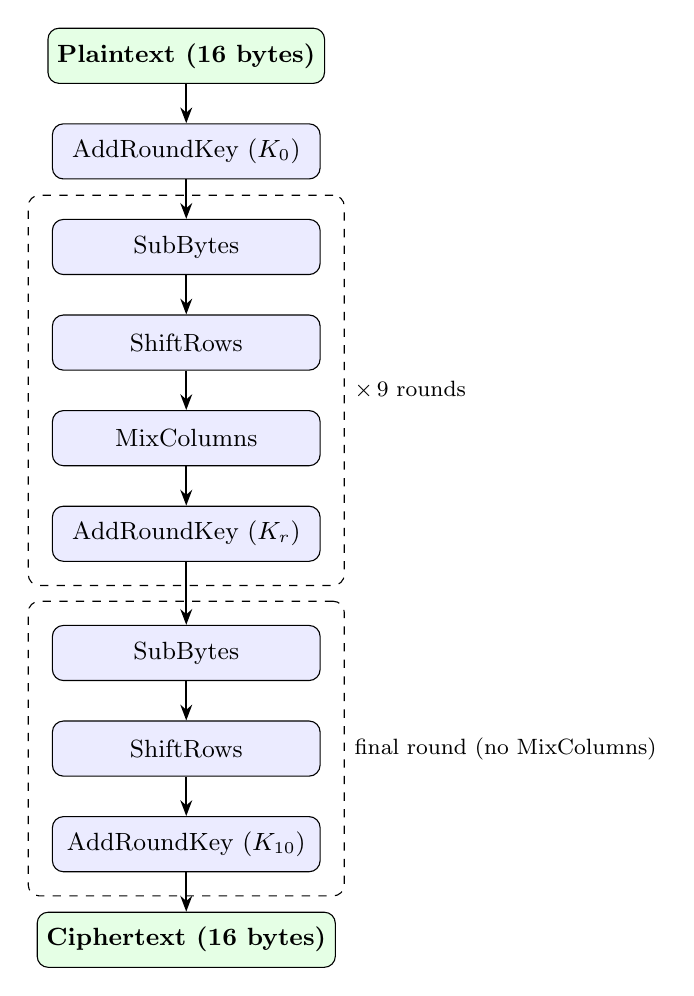
\begin{tikzpicture}[node distance=5mm]
  \node[io] (pt) {Plaintext (16 bytes)};
  \node[op,below=of pt] (ark0) {AddRoundKey ($K_0$)};
  \node[op,below=of ark0] (sb) {SubBytes};
  \node[op,below=of sb] (sr) {ShiftRows};
  \node[op,below=of sr] (mc) {MixColumns};
  \node[op,below=of mc] (ark) {AddRoundKey ($K_r$)};
  \node[op,below=8mm of ark] (fsb) {SubBytes};
  \node[op,below=of fsb] (fsr) {ShiftRows};
  \node[op,below=of fsr] (fark) {AddRoundKey ($K_{10}$)};
  \node[io,below=of fark] (ct) {Ciphertext (16 bytes)};
  \foreach \a/\b in {pt/ark0,ark0/sb,sb/sr,sr/mc,mc/ark,ark/fsb,fsb/fsr,fsr/fark,fark/ct}
    \draw[flow] (\a) -- (\b);
  % round-1..9 bracket
  \begin{scope}[on background layer]
    \node[draw,dashed,rounded corners,fit=(sb)(ark),inner sep=3mm,label=right:{\footnotesize $\times\,9$ rounds}] {};
    \node[draw,dashed,rounded corners,fit=(fsb)(fark),inner sep=3mm,label=right:{\footnotesize final round (no MixColumns)}] {};
  \end{scope}
\end{tikzpicture}
\caption{The AES-128 encryption flow. Nine full rounds, then a final round.}
\end{figure}

\noindent\textbf{Known-answer check.} With key \texttt{000102\dots0E0F} and
plaintext \texttt{001122\dots EEFF}, the code produces ciphertext
\texttt{\AEScipher}, matching the FIPS 197 example.

%====================================================================
\section{The AES S-box}
%====================================================================

SubBytes replaces every byte through one fixed 16$\times$16 lookup table --- the
only non-linear step in AES. The heatmap shades each entry by its value (light =
low, dark = high); rows are the high nibble, columns the low nibble.

\begin{figure}[H]\centering
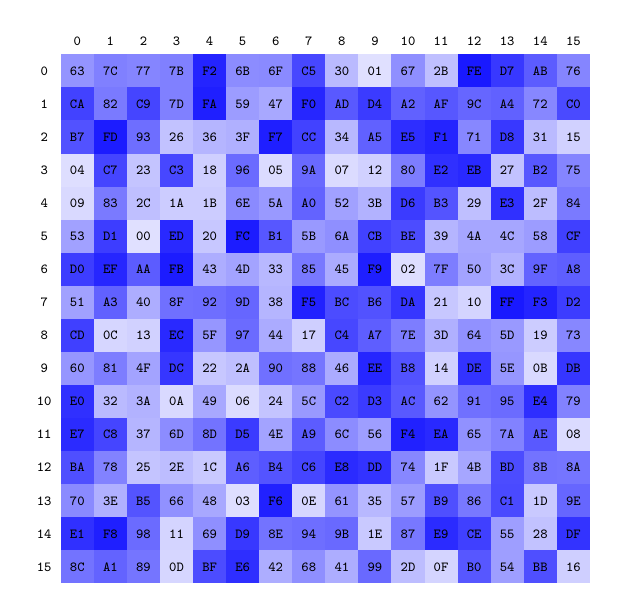
\begin{tikzpicture}[scale=0.42]
  \AESsboxgrid
  \foreach \c in {0,...,15} \node[font=\tiny] at (\c+0.5,0.4) {\texttt{\c}};
  \foreach \r in {0,...,15} \node[font=\tiny] at (-0.5,-\r-0.5) {\texttt{\r}};
\end{tikzpicture}
\caption{AES S-box. Bijective (a permutation of all 256 bytes). Fixed points: \AESfixed.}
\end{figure}

A good substitution box is a bijection with no fixed point ($S(x)=x$) and no
opposite fixed point; the AES S-box satisfies this, which is one reason a
one-byte change never ``stays put''.

%====================================================================
\section{Diffusion --- how one bit spreads}
%====================================================================

Flip a single bit of the plaintext and compare, after every round, against the
unmodified encryption. Two measurements: how many of the 16 \textbf{bytes}
differ, and the Hamming distance in \textbf{bits} (out of 128). Full diffusion
means about half the bits (64) differ --- an attacker learns nothing from the
output about which bit changed.

\begin{figure}[H]\centering
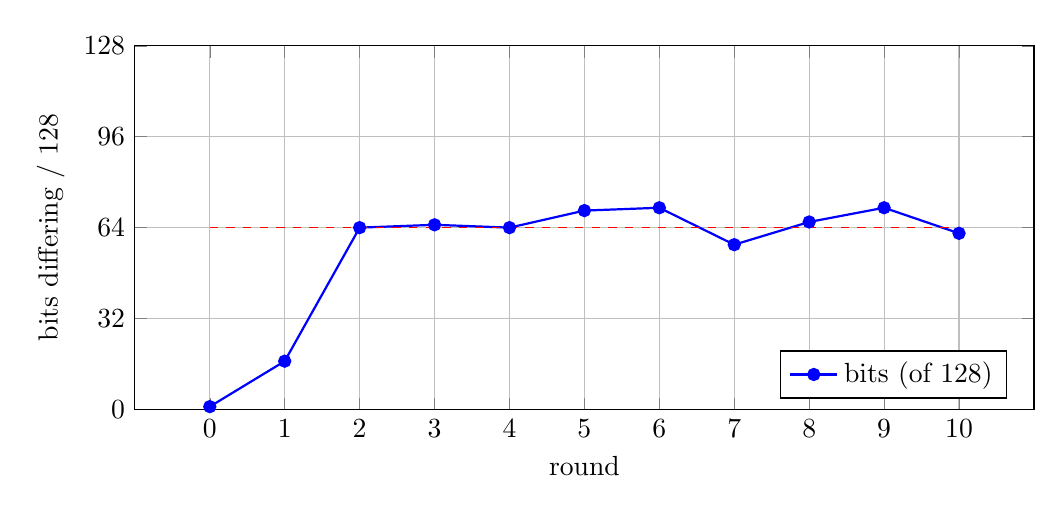
\begin{tikzpicture}
\begin{axis}[width=13cm,height=6.2cm,ymin=0,ymax=128,
   xlabel={round},ylabel={bits differing / 128},
   xtick={0,1,2,3,4,5,6,7,8,9,10},ytick={0,32,64,96,128},
   grid=both,legend pos=south east,legend cell align=left]
  \addplot[blue,mark=*,thick] coordinates {\AESavalanche};
  \addlegendentry{bits (of 128)}
  \draw[red,dashed] (axis cs:0,64) -- (axis cs:10,64);
\end{axis}
\end{tikzpicture}
\caption{AES avalanche effect. One flipped input bit reaches \AESbitsreached\ bits
after round~1 and about half (\AESbitsfull) by round~2.}
\end{figure}

\begin{figure}[H]\centering
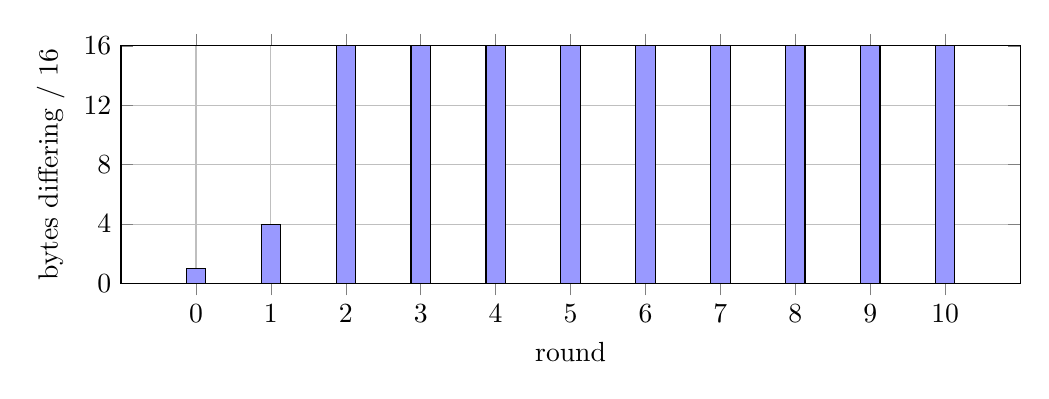
\begin{tikzpicture}
\begin{axis}[width=13cm,height=4.6cm,ymin=0,ymax=16,
   xlabel={round},ylabel={bytes differing / 16},
   xtick={0,1,2,3,4,5,6,7,8,9,10},ytick={0,4,8,12,16},
   grid=both,ybar,bar width=7pt]
  \addplot[fill=blue!40] coordinates {\AESbytes};
\end{axis}
\end{tikzpicture}
\caption{Byte diffusion: MixColumns spreads one changed byte to a full column
(4 bytes) in round~1, and ShiftRows + MixColumns reach all 16 bytes by round~2.}
\end{figure}

%====================================================================
\section{SM4 at a glance}
%====================================================================

SM4 is the Chinese national block cipher (GB/T 32907). It also works on 128-bit
blocks, but is built as a \textbf{32-round Feistel-like network} on four 32-bit
words $X_0,X_1,X_2,X_3$. Each round replaces the oldest word:
\[
  X_{i+4} \;=\; X_i \,\oplus\, T\!\left(X_{i+1}\oplus X_{i+2}\oplus X_{i+3}\oplus rk_i\right),
\]
where $T = L(\tau(\cdot))$: $\tau$ applies the S-box to each of the four bytes,
and $L$ mixes them with rotations $L(b)=b\oplus(b\lll2)\oplus(b\lll10)\oplus(b\lll18)\oplus(b\lll24)$.

\begin{figure}[H]\centering
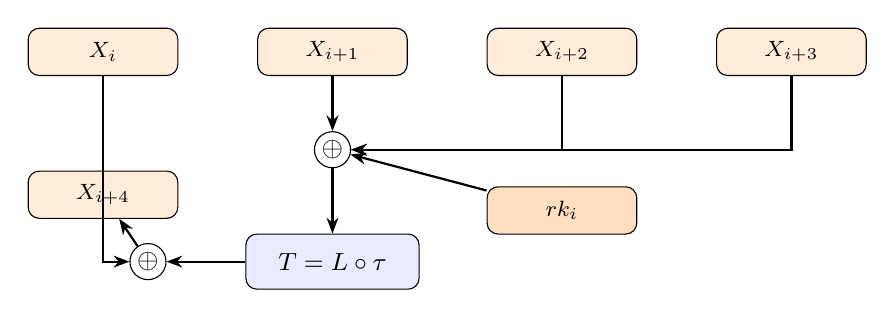
\begin{tikzpicture}[node distance=6mm and 10mm]
  \node[keyb] (x0) {$X_i$};
  \node[keyb,right=of x0] (x1) {$X_{i+1}$};
  \node[keyb,right=of x1] (x2) {$X_{i+2}$};
  \node[keyb,right=of x2] (x3) {$X_{i+3}$};
  \node[keyb,fill=orange!25,below=14mm of x2] (rk) {$rk_i$};
  \node[draw,circle,inner sep=1pt,below=7mm of x1] (xor1) {$\oplus$};
  \node[op,below=20mm of x1,minimum width=2.2cm] (T) {$T = L\circ\tau$};
  \node[draw,circle,inner sep=1pt,left=of T] (xor2) {$\oplus$};
  \node[keyb,below=12mm of x0] (nx) {$X_{i+4}$};
  \draw[flow] (x1) -- (xor1); \draw[flow] (x2) |- (xor1); \draw[flow] (x3) |- (xor1);
  \draw[flow] (rk) -- (xor1);
  \draw[flow] (xor1) -- (T);
  \draw[flow] (T) -- (xor2);
  \draw[flow] (x0) |- (xor2);
  \draw[flow] (xor2) -- (nx);
\end{tikzpicture}
\caption{One SM4 round. After 32 rounds the ciphertext is $(X_{35},X_{34},X_{33},X_{32})$.}
\end{figure}

\noindent\textbf{Known-answer check.} With key and plaintext both
\texttt{0123\dots3210}, the code produces \texttt{\SMfourcipher}.

\begin{figure}[H]\centering
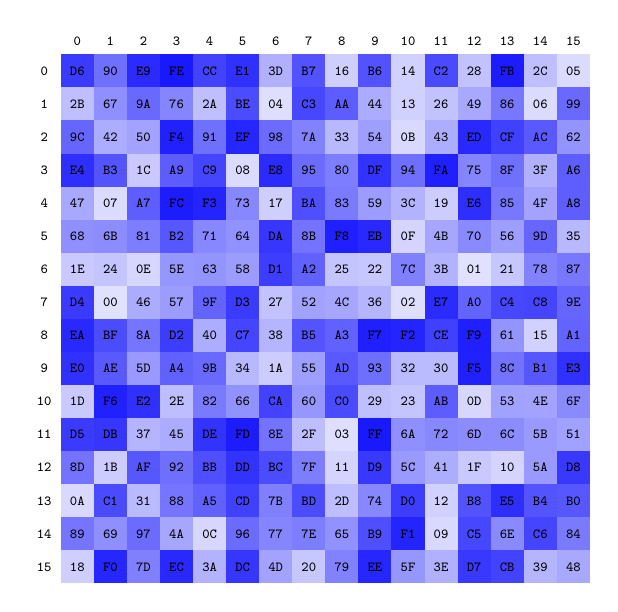
\begin{tikzpicture}[scale=0.42]
  \SMfoursboxgrid
  \foreach \c in {0,...,15} \node[font=\tiny] at (\c+0.5,0.4) {\texttt{\c}};
  \foreach \r in {0,...,15} \node[font=\tiny] at (-0.5,-\r-0.5) {\texttt{\r}};
\end{tikzpicture}
\caption{SM4 S-box, shaded by value. Bijective. Fixed points: \SMfourfixed.}
\end{figure}

\begin{figure}[H]\centering
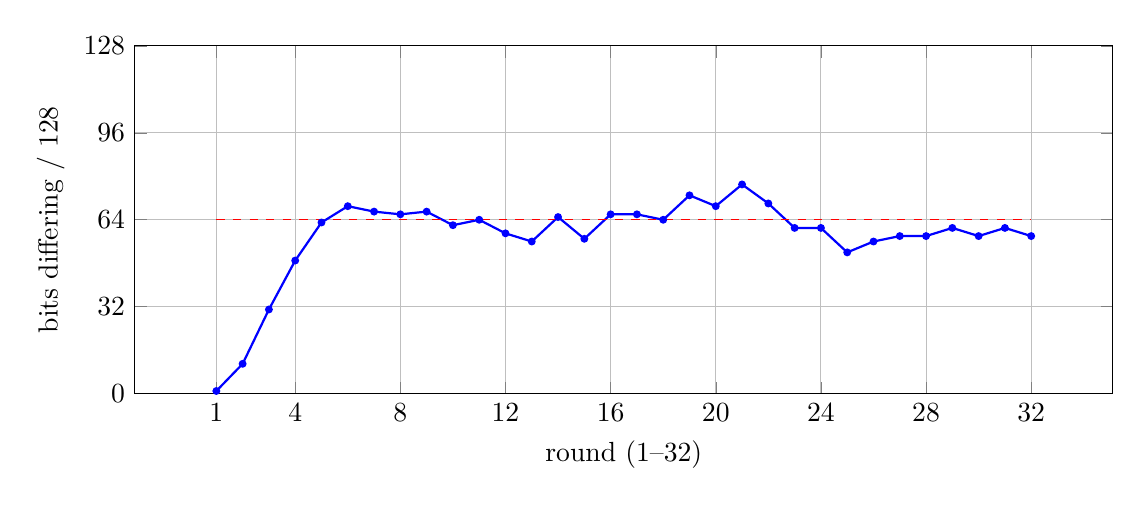
\begin{tikzpicture}
\begin{axis}[width=14cm,height=6cm,ymin=0,ymax=128,
   xlabel={round (1--32)},ylabel={bits differing / 128},
   xtick={1,4,8,12,16,20,24,28,32},ytick={0,32,64,96,128},
   grid=both]
  \addplot[blue,mark=*,mark size=1pt,thick] coordinates {\SMfouravalanche};
  \draw[red,dashed] (axis cs:1,64) -- (axis cs:32,64);
\end{axis}
\end{tikzpicture}
\caption{SM4 avalanche effect across its 32 rounds. Diffusion builds more
gradually than AES because each round changes only one 32-bit word.}
\end{figure}

%====================================================================
\section{AES vs.\ SM4 --- summary}
%====================================================================

\begin{table}[H]\centering
\begin{tabular}{@{}lll@{}}
\toprule
 & \textbf{AES-128} & \textbf{SM4} \\
\midrule
Block / key size & 128 / 128 bits & 128 / 128 bits \\
Structure        & Substitution--permutation & Feistel-like network \\
Rounds           & 10 & 32 \\
State            & 4$\times$4 bytes & four 32-bit words \\
Non-linear step  & S-box (SubBytes) & S-box ($\tau$) \\
Linear step      & ShiftRows + MixColumns & rotations $L$ \\
S-box fixed points & \AESfixed & \SMfourfixed \\
\bottomrule
\end{tabular}
\caption{Side-by-side structure, with S-box fixed points measured from the code.}
\end{table}

\vfill
\noindent\footnotesize\emph{Reproducibility:} rerun \texttt{python make\_analysis.py}
to regenerate \texttt{analysis/data.tex} and rebuild this PDF. All figures are
redrawn from the current \texttt{src/} implementations.

\end{document}
